\documentclass[10pt]{article}

\usepackage[margin=0.75in]{geometry}
\usepackage{amsmath, amssymb}
\usepackage{graphicx}
\usepackage[T1]{fontenc}
\usepackage{inconsolata}
\usepackage{titlesec}
\usepackage{fancyhdr}
\usepackage{microtype}
\usepackage{array}
\usepackage{enumitem}
\usepackage{tikz}
\usetikzlibrary{arrows.meta,calc}

\graphicspath{{../}}

\setlength{\parindent}{0pt}
\setlength{\parskip}{4pt}
\renewcommand{\baselinestretch}{1.05}

\titleformat{\section}{\ttfamily\normalsize\bfseries\MakeUppercase}{\thesection}{0.6em}{}
\titlespacing*{\section}{0pt}{5pt}{1pt}
\titleformat{\subsection}{\ttfamily\small\MakeUppercase}{\thesubsection}{0.6em}{}
\titlespacing*{\subsection}{0pt}{3pt}{1pt}

\setlist[itemize]{
  leftmargin=1.15em,
  itemsep=0.7pt,
  topsep=1pt,
  parsep=0pt,
  partopsep=0pt
}

\newcommand{\tightitem}[1]{\item #1}

\tikzset{
  steel/.style={draw=black, line width=0.65pt, fill=black!8},
  bolt/.style={draw=black, line width=0.65pt, fill=black!38},
  washer/.style={draw=black, line width=0.65pt, fill=black!18},
  leader/.style={draw=black, line width=0.4pt, -{Latex[length=1.5mm]}},
  force/.style={draw=black, line width=1.0pt, -{Latex[length=2.2mm]}},
  shearplane/.style={draw=black, line width=0.8pt, densely dashed},
  glabel/.style={font=\ttfamily\scriptsize, inner sep=1pt, fill=white}
}

\pagestyle{fancy}
\fancyhf{}
\renewcommand{\headrulewidth}{0pt}
\renewcommand{\footrulewidth}{0.5pt}
\fancyfoot[L]{\ttfamily\footnotesize A325-BOLTS}
\fancyfoot[C]{\ttfamily\footnotesize REV \today}
\fancyfoot[R]{\ttfamily\footnotesize \thepage}

\begin{document}

\noindent
\includegraphics[height=0.7cm]{logo}\hfill
{\ttfamily\small\bfseries\MakeUppercase{ASTM A325-N Bolts --- Use + Inspection}}\quad
{\ttfamily\footnotesize\today}
\vspace{3pt}\hrule\vspace{3pt}

\section{Code Basis}

{\ttfamily\footnotesize
\setlength{\tabcolsep}{2pt}
\begin{tabular}{@{}p{0.14\textwidth}p{0.29\textwidth}p{0.24\textwidth}p{0.27\textwidth}@{}}
IBC 2018 &
ANSI/AISC 360-16, SECTION N5.6 &
RCSC 2014, SECTION 9.1 &
CURRENT: ASTM F3125 GRADE A325
\end{tabular}
}

\section{Connection Use}

\noindent
\begin{minipage}[t]{0.63\textwidth}
\vspace{0pt}
\centering
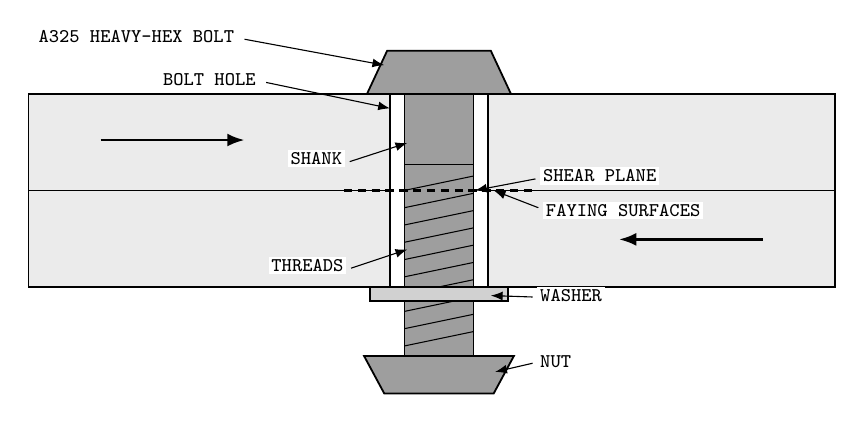
\begin{tikzpicture}[x=0.72in,y=0.72in]
  % Connected steel plies and bolt holes.
  \draw[steel] (0.15,1.45) rectangle (5.75,2.12);
  \draw[steel] (0.15,0.78) rectangle (5.75,1.45);
  \fill[white] (2.66,0.78) rectangle (3.34,2.12);
  \draw[line width=0.45pt] (2.66,0.78) -- (2.66,2.12);
  \draw[line width=0.45pt] (3.34,0.78) -- (3.34,2.12);

  % Heavy-hex head, shank, threaded portion, washer, and nut.
  \draw[bolt] (2.50,2.12) -- (2.64,2.42) -- (3.36,2.42) --
              (3.50,2.12) -- cycle;
  \draw[bolt] (2.76,1.63) rectangle (3.24,2.12);
  \draw[bolt] (2.76,0.30) rectangle (3.24,1.63);
  \foreach \y in {0.37,0.49,...,1.57} {
    \draw[line width=0.38pt] (2.76,\y) -- (3.24,\y+0.10);
  }
  \draw[washer] (2.52,0.68) rectangle (3.48,0.78);
  \draw[bolt] (2.48,0.30) -- (2.62,0.04) -- (3.38,0.04) --
              (3.52,0.30) -- cycle;

  % Shear actions and plate interface.
  \draw[force] (0.65,1.80) -- (1.65,1.80);
  \draw[force] (5.25,1.11) -- (4.25,1.11);
  \draw[shearplane] (2.34,1.45) -- (3.66,1.45);

  % Graphic labels.
  \node[glabel,anchor=east] at (1.60,2.52) {A325 HEAVY-HEX BOLT};
  \draw[leader] (1.65,2.50) -- (2.62,2.32);
  \node[glabel,anchor=east] at (1.75,2.22) {BOLT HOLE};
  \draw[leader] (1.80,2.20) -- (2.66,2.02);
  \node[glabel,anchor=east] at (2.35,1.67) {SHANK};
  \draw[leader] (2.38,1.65) -- (2.78,1.78);
  \node[glabel,anchor=east] at (2.36,0.93) {THREADS};
  \draw[leader] (2.39,0.91) -- (2.78,1.04);
  \node[glabel,anchor=west] at (3.68,0.72) {WASHER};
  \draw[leader] (3.65,0.71) -- (3.36,0.72);
  \node[glabel,anchor=west] at (3.68,0.26) {NUT};
  \draw[leader] (3.65,0.25) -- (3.39,0.19);
  \node[glabel,anchor=west] at (3.70,1.55) {SHEAR PLANE};
  \draw[leader] (3.67,1.53) -- (3.25,1.45);
  \node[glabel,anchor=west] at (3.72,1.31) {FAYING SURFACES};
  \draw[leader] (3.69,1.33) -- (3.38,1.45);
\end{tikzpicture}
\end{minipage}\hfill
\begin{minipage}[t]{0.34\textwidth}
\vspace{0pt}
\setlength{\fboxsep}{5pt}
\fbox{\parbox{\dimexpr\linewidth-2\fboxsep-2\fboxrule\relax}{
  {\ttfamily\small\bfseries A325-N\par}
  \vspace{2pt}
  {\ttfamily\footnotesize\bfseries
  BEARING-TYPE CONNECTION\par
  THREADS INCLUDED IN SHEAR PLANE\par}
}}

\vspace{5pt}
{\ttfamily\scriptsize
\begin{tabular}{@{}>{\bfseries}l@{\ }p{1.62in}@{}}
A325-X $\rightarrow$ & THREADS EXCLUDED FROM SHEAR PLANE \\[2pt]
A325-SC $\rightarrow$ & SLIP-CRITICAL CONNECTION
\end{tabular}
}

\vspace{5pt}
{\footnotesize N, X, and SC describe connection use---not different bolt materials.}
\end{minipage}

\vspace{2pt}
\noindent
\begin{minipage}[t]{0.48\textwidth}
\vspace{0pt}
\section{Typical Uses}

\footnotesize
\begin{itemize}
  \tightitem{Beam shear connections.}
  \tightitem{Beam and column splices.}
  \tightitem{Gusset and bracing connections.}
  \tightitem{End-plate connections.}
  \tightitem{Steel-to-steel joints carrying shear or combined shear and tension.}
\end{itemize}

\setcounter{section}{4}
\section{Not Required Solely Because Bolt Is A325-N}

\footnotesize
\begin{itemize}
  \tightitem{Measurement of actual bolt clamping force.}
  \tightitem{Generic torque-wrench calibration.}
  \tightitem{AWS D1.1 certification for the bolt installer.}
\end{itemize}
\end{minipage}\hfill
\begin{minipage}[t]{0.49\textwidth}
\vspace{0pt}
\setcounter{section}{3}
\section{Inspection --- Typical Snug-Tight A325-N Joint}

{\ttfamily\footnotesize\bfseries PRIOR TO BOLTING}

\footnotesize
\begin{itemize}
  \tightitem{Confirm specified bolt, nut, and washer components.}
  \tightitem{Confirm required ASTM markings, grade, type, diameter, and length.}
  \tightitem{Confirm proper storage and suitability for installation.}
  \tightitem{Confirm holes and connected steel plies meet joint requirements.}
\end{itemize}

{\ttfamily\footnotesize\bfseries AFTER ASSEMBLY}

\footnotesize
\begin{itemize}
  \tightitem{Confirm connected plies are in firm contact.}
  \tightitem{Confirm washers are installed where required.}
  \tightitem{Confirm every bolt is snug-tight and the nut cannot be removed without a wrench.}
  \tightitem{Document acceptance or rejection of the connection.}
\end{itemize}
\end{minipage}

\setcounter{section}{5}

\vspace{5pt}
\setlength{\fboxsep}{5pt}
\noindent\fbox{\parbox{\dimexpr\textwidth-2\fboxsep-2\fboxrule\relax}{
{\ttfamily\footnotesize\bfseries
PRETENSIONED OR SLIP-CRITICAL JOINTS REQUIRE ADDITIONAL,
INSTALLATION-METHOD-SPECIFIC INSPECTION. A325-N ALONE
DOES NOT REQUIRE THAT ADDITIONAL INSPECTION.}
}}

\end{document}
